\chapter{Relationship between  $B_1$-EPG, EPT and VPT graph classes}
\label{cap:v}

\begin{flushright}
\begin{minipage}[t][0cm][b]{0.47\textwidth}
\emph{
A Matemática não mente. Mente quem faz mau uso dela.}
\end{minipage}

\rule[0cm]{7cm}{0.03cm}%{largura}{espessura}

Albert Einstein
\end{flushright}

Esse capítulo apresenta como resultado principal que todo grafo Cordal $B_1$-EPG está simultaneamente nas classes de grafo VPT e EPT. Em particular, descrevemos estruturas que sempre estão presentes em grafos que não admitem uma representação $B_1$-EPG-Helly e assim definimos alguns conjuntos de subgrafos que delimitam subfamílias Helly.   
Além disso, esse capítulo também apresenta caracterizações para algumas famílias não-triviais de grafos que estão propriamente contidas em   $B_1$-EPG-Helly, nomeadamente essas famílias são compostas pelos grafos Bipartidos, Blocos, Cactus e Linha de Bipartido. 



\section{Discussão Inicial}

Modelos baseados em intersecção de caminhos podem ser considerados basicamente sob dois pontos de vista, o primeiro considera as intersecções em vértices e o segundo em arestas. Casos onde os caminhos são hospedados em uma árvore aparecem primeiro na literatura, veja por exemplo~\cite{gavril1978recognition, golumbic1985edge, golumbic1985}.  Representações usando caminhos sobre uma grade foram considerados mais tarde, ver~\cite{golumbic2009,golumbic2013, golumbic2013intersection}. A seguir detalharemos os modelos de intersecção que serão estudados neste capítulo. %More details on each intersection model will be given in the following text.

 Seja $P$ uma família de caminhos sobre uma árvore hospedeira $T$. Dois tipos de grafos de intersecção do par  $<P,T>$ são definidos, denotaremos esses como grafos VPT e EPT.
Os \textit{Grafos de Intersecção de Arestas} de $P$, EPT(P), possuem  vértices que correspondem aos membros de $P$, e dois vértices são  adjacentes em EPT(P) se e somente se os caminhos correspondentes em $P$ compartilham pelo menos uma aresta em $T$. Similarmente, os \textit{Grafos de Intersecção de Vértices} de $P$, VPT(P), possuem vértices que correspondem aos membros de  $P$, e dois vértices são adjacentes em VPT(P) se e somente se os caminhos correspondentes em  $P$ compartilham pelo menos um vértice em $T$. Em qualquer dos modelos considerados, sempre existe uma função de bijeção entre as intersecções dos caminhos e as adjacências dos vértices correspondentes. 


Grafos VPT e EPT definem famílias incomparáveis de grafos. Entretanto, quando o grau máximo da árvore hospedeira é restrito a três, então a família dos grafos VPT coincide com a família dos grafos EPT~ \cite{golumbic1985edge% \cite{alcon2010necessary
}. Também é conhecido que qualquer grafo Cordal EPT é também um grafo VPT (see~\cite{syslo1985triangulated}). Recordando também que outro resultado conhecido na literatura é o de que os grafos Cordais são os grafos de intersecção em vértices de subárvores de uma árvore, ver~\cite{gavril1974intersection}.


\textit{Grafos de Intersecção de Caminhos sobre uma Grade} são chamados de \textit{grafos EPG}. 

Em \cite{golumbic2009}, o autor provou que todos os grafos possuem uma representação EPG, e iniciou o estudo das subclasses definidas pela limitação do número de vezes que qualquer caminho utilizado na representação pode dobrar. Grafos admitindo uma representação onde caminhos possuem no máximo  $k$ mudanças de direção (dobras) foram chamados de grafos $B_k$-EPG. 
 Em particular, quando os caminhos possuem no máximo uma dobra então temos os grafos \textit{ $B_1$-EPG}, também conhecidos como grafos EPG de  \textit{dobra simples}.

Uma questão pertinente no contexto de grafos de intersecção de caminhos é como segue: dadas duas classes de de grafos de intersecção de caminhos,  a primeira cujo hospedeiro é uma árvore e a segunda cujo hospedeiro é uma grade, existe uma intersecção ou um relacionamento de continência entre essas classes? O que sabemos sobre isso?

Nesse capítulo iremos explorar os grafos  $B_1$-EPG, em particular os grafos diamante-livre e os grafos Cordais. Trabalharemos principalmente sobre questões a respeito da relação de contenção entre as classes de grafos VPT, EPT e $B_1$-EPG.

Uma coleção de conjuntos satisfaz a   \textit{propriedade Helly} quando toda subcoleção que é mutuamente intersectante possui pelo menos um elemento em comum. Quando essa propriedade é satisfeita pelo conjunto de vértices (ou arestas) dos caminhos utilizados na representação, então temos uma representação Helly. Grafos   $B_1$-EPG-Helly foram estudados em~\cite{bornstein2019}, que mostraram que todo grafo admite uma representação Helly e também que o problema de reconhecer grafos $B_1$-EPG-Helly é $NP$-completo.  

É conhecido que nem todo grafo $B_1$-EPG admite uma representação  $B_1$-EPG-Helly. Estamos interessados em determinar os subgrafos que são grafos
$B_1$-EPG porém não admitem uma representação  Helly $B_1$-EPG. Nesse capítulo, descrevemos estruturas que estarão presentes em qualquer desses subgrafos, além do mais, também apresentamos novas subclasses de grafos  $B_1$-EPG-Helly. Ademais, delimitamos novas subclasses $B_1$-EPG-Helly e damos alguns  conjuntos de subgrafos que delimitam subfamílias Helly.
\section{Definições e Resultados Técnicos}

O \textit{conjunto de vértices} e o \textit{conjunto de arestas} de um grafo  $G$ são denotados por $V(G)$ e $E(G)$, respectivamente.  Dado um vértice  $v\in V(G)$,  $N(v)$ e $N[v]$ representam a   \textit{vizinhança} aberta e fechada de  $v$ em $G$, respectivamente. 
Para um subconjunto  $S \subseteq V(G)$,  $G[S]$ é o subgrafo de $G$ induzido por $S$.
 Se $\mathcal{F}$ é uma família qualquer de grafos, dizemos que $G$ é  \textit{$\mathcal{F}$-livre} se $G$ não possui subgrafo induzido isomorfo a um membro de $\mathcal{F}$.
 Um \textit{ciclo},  denotado por $C_n$, é uma sequência de vértices distintos  $v_1, \dots , v_n, v_1$  onde $v_i \neq v_j$ for $i \neq j$ e $(v_i, v_i + 1) \in E(G)$, tal que $n \geq 3$. Uma \textit{corda} é uma aresta que está entre dois vértices não-consecutivos em uma sequência de vértices de um ciclo. Um \textit{ciclo induzido}  ou \textit{ciclo sem corda} é um ciclo que não possui corda, nesse capítulo todo ciclo induzido será chamado simplesmente de  \textit{ciclo}. Um grafo  $G$ formado por um ciclo induzido $H$ mais um único vértice universal  $v$ conectado a todos vértices de $H$ é chamado  \textit{grafo roda}. Se o grafo roda possui $n$ vértices, ele é denotado por $n$-roda. 

O grafo $k$\textit{-sol} $S_k$, $k \geq 3$, consiste de 
$2k$ vértices, um conjunto independente $X = \{x_1, \dots, x_k\}$ e uma clique $Y = \{y_1, \dots, y_k\}$, e um conjunto de arestas $E_1 \cup E_2$, onde $E_ 1=\{ (x_1,y_1); (y_1, x_2); (x_2, y_2); (y_2, x_3); \dots , (x_k, y_k); (y_k, x_1) \}$ forma o ciclo externo e $E_2= \{(y_i, y_j) |i\neq j\}$ forma uma clique interna.

Um grafo é $ B_k$-EPG se ele admite uma representação EPG em que cada caminho possui no máximo $k$ dobras. Quando $ k = 1 $ dizemos que essa é uma representação \emph{ EPG de dobra simples} ou simplesmente uma representação  $B_1$-EPG. 
Uma \textit{clique} é um conjunto de vértices mutuamente adjacentes, enquanto
um \textit{conjunto independente} é um conjunto de vértices não mutuamente adjacentes entre si.
 Dada uma representação EPG de um grafo  $G$, identificaremos cada vértice  $v$ de $G$ com o correspondente caminho  $P_{v}$ da grade, utilizado na representação. Adequadamente, por exemplo, diremos que um vértices de  $G$ cobre ou contem alguma aresta da grade (significando que o correspondente caminho faz isso), ou que o conjunto de caminhos da representação induz um subgrafo de $G$ (significando que o correspondente conjunto de vértices faz isso, na verdade). 

Em uma representação $B_1$-EPG, uma clique $K$ é dita ser uma \textit{clique-aresta} se todos os vértices de $K$ compartilham pelo menos uma aresta comum da grade (ver Figura~\ref{fig:cliquesRepresentation}(a)).
 Uma \textit{garra da grade} é um conjunto de três arestas da grade, incidentes no mesmo ponto da grade, que é chamado o \textit{centro da garra}. As duas arestas da garra que tem a mesma direção formam a  \textit{ base da garra}. Se $K$ não é uma clique-aresta, então existe uma garra da grade   (e somente uma) tal que os vértices de  $K$ são aqueles que contem exatamente duas das três arestas dessa garra; tal clique é chamada de   \textit{clique-garra} \cite{golumbic2009} (ver Figura~\ref{fig:cliquesRepresentation}(b)).

    

\begin{figure}[h]
  \centering
  \begin{tabular}{  p{4.5cm} p{0.7cm} p{4cm} }
    %\centering
    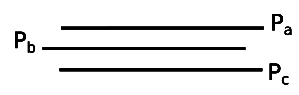
\includegraphics[width=4.5cm]{img/edge-clique.png} & &
    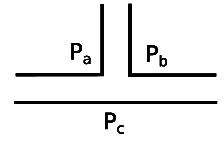
\includegraphics[width=3.5cm]{img/claw-clique.png}%b1EpgTransparenteGrade2
    \\
    \footnotesize %\centering 
    (a)  \footnotesize Representation of a clique as edge-clique. && \footnotesize (b) Representation  of a clique as claw-clique.\\
  \end{tabular}

 \caption{Examples of clique representations.} \label{fig:cliquesRepresentation}
\end{figure}


















% \begin{figure}[h]
%   \centering
%   \begin{tabular}{  p{4cm} p{0.7cm} p{4cm} }
%     %\centering
%     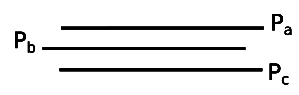
\includegraphics[width=4.5cm]{img/edge-clique.png} & &
%     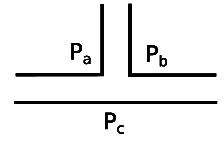
\includegraphics[width=3.5cm]{img/claw-clique.png}%b1EpgTransparenteGrade2
%     \\
%     \footnotesize %\centering 
%     (a)  \footnotesize Representação de uma  clique como clique-aresta. && \footnotesize (b) Representação de uma  clique como clique-garra.\\
%   \end{tabular}

%  \caption{Exemplos de representações de clique.} \label{fig:cliquesRepresentation}
% \end{figure}    

Note que se três vértices induzem uma clique-garra, então exatamente dois deles dobram no centro da garra correspondente na grade, e o terceiro contem a base da garra.
Além disso, qualquer outro vértice adjacente aos três deve conter duas das arestas dessa garra, então o seguinte lema é válido.

\begin{lema}\label{lem:cliquesMaximais}
Se três vértices estão juntos em mais que uma  clique maximal do grafo $G$, então em qualquer representação $B_1$-EPG de $G$ esses três vértices não formam uma  clique-garra.
\end{lema}

\begin{figure}[ht]
  \centering
  \begin{tabular}{  p{5cm} p{0.7cm} p{5cm} }
    %\centering
    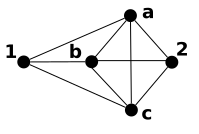
\includegraphics[width=3.5cm]{img/lemaClaw2Maximais} & &
    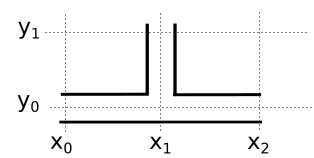
\includegraphics[width=5.5cm]{img/claw2}
    \\
    \footnotesize %\centering 
    (a)  \footnotesize Examplo de duas cliques maximais compartilhando vértices. && \footnotesize (b) Representação de uma clique-garra na grade.\\
  \end{tabular}

 \caption{Vértices representados por uma garra  estão presentes em uma única clique maximal.} \label{fig:lemaClaw2Maximais}
\end{figure}

Em Asinowski et al. \cite{ries2009} foi provado o seguinte lema para grafos $C_4$-livre.

\begin{lema} \cite{ries2009} \label{lem:lemaBRies2009}
Seja $G$ um grafo $B_1$-EPG. Se $G$ é $C_4$-livre, então existe uma representação $B_1$-EPG de $G$ tal que toda clique-garra maximal $K$ é representada sobre uma  garra da grade cuja base é coberta unicamente por vértices de $K$.
\end{lema}


Temos obtido o seguinte resultado, similar para grafos diamante-livre. Um \textit{diamante} é um grafo  $G$ com conjunto de vértices  $V(G) = \{a, b, c, d\}$ e conjunto de arestas $E(G)=\{ab, ac,bc, bd,cd\}$ (ver Figura~\ref{fig:diamond}). %A graph is diamante-livre if it does not contain a diamante as induced subgraph.

 \begin{figure}[htb]	
 \center%6.3
 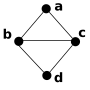
\includegraphics[width=2.2cm]{./img/diamond.png}
 \caption{Diamond graph.}
\label{fig:diamond}
\end{figure}  
 


\begin{lema}\label{lem:b1epgDiamondFree}
Seja $G$ um grafo $B_1$-EPG. Se $G$ é diamante-livre, então em qualquer representação $B_1$-EPG de $G$,  toda  clique-garra maximal $K$ é representada sobre uma garra da grade cujas arestas são cobertas somente por  vértices de $K$.
\end{lema}

\begin{proof}Seja $K$ uma  clique maximal que é uma clique-garra em uma dada representação $B_1$-EPG de $G$. Então existem três  vértices de $K$ que induzem uma  clique-garra $K'$ sobre a mesma garra da grade que $K$. Assuma, de forma a derivar uma contradição, que um vértice $v\notin K$ cobre alguma aresta da garra. Claramente, $v$ deve cobrir somente uma das arestas. Portanto $v$ e os vértices de $K'$ induzem um  diamante, uma contradição.
\end{proof}


% \begin{defi} \label{defi:tortasFrame}

Seja $ Q $ uma grade e sejam $ (a_1, b),$ $(a_2, b),$ $(a_3, b),$ $(a_4, b)$ uma $4$-estrela centrada em $b$ como ilustrado na Figura~\ref{fig:piesInGrid}(a). Seja $ \mathcal{P} = \{P_1, \dots , P_4\}$ uma coleção de quatro caminhos cada um contendo um diferente par de arestas da $4$-estrela.
%exactly two edges of the $4$-estrela:
Seguindo \cite{golumbic2009}, dizemos que esses quatro caminhos formam:

\begin{itemize}
\item uma \emph{torta verdadeira}  quando cada um possui uma dobra em  $b$, Figura~\ref{fig:piesInGrid}(b); e
\item uma \emph {torta falsa} quando exatamente dois dos caminhos dobram em  $b$ e eles não compartilham aresta da $4$-estrela, Figura~\ref{fig:piesInGrid}(c). %contain bends, while the remaining two do not share an edge. 

\begin{figure}[htb]
  \centering
%segundo bloco de figuras
  \begin{tabular}{c c c c c }
    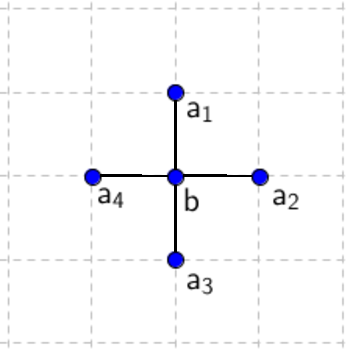
\includegraphics[width=3.5cm]{img/disposicaoTortaGrid3.pdf}    
    & &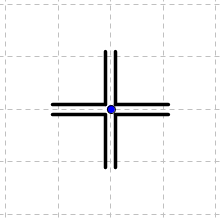
\includegraphics[width=3.5cm]{img/truePieGrid} 
    & &
 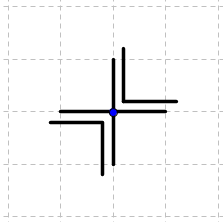
\includegraphics[width=3.5cm]{img/falsePieGrid} \\%[\abovecaptionskip]
    {\footnotesize (a) 4-estrela em uma grade.}  & &  {\footnotesize (b) Torta verdadeira.} & & {\footnotesize (c) Torta falsa.} 
  \end{tabular}
  \caption{Representação $B_{1}$-EPG do ciclo induzido de tamanho  4 como tortas, com ênfase no centro $b$.}\label{fig:piesInGrid}
\end{figure} 

%\vspace{-0.5cm}
\end{itemize}
% \end{defi}

Claramente se quatro caminhos de uma representação $B_1$-EPG de $G$ formam uma torta, então os vértices correspondentes induzem um $4$-ciclo em $G$. % The converse implication is also true (see~\cite{golumbic2009}). 
O seguinte resultado pode ser facilmente provado. Dizemos que um conjunto de caminhos forma uma garra quando cada par de arestas da  garra está coberto por algum dos caminhos.

\begin{lema}\label{lem:twogarraNotSameCenterInCordal}
Em qualquer representação $B_1$-EPG de um grafo $G$, um conjunto de caminhos formando duas diferentes garras centradas no mesmo ponto da grade contem quatro caminhos formando também uma torta verdadeira ou uma torta falsa. Portanto, em qualquer representação $B_1$-EPG de um grafo Cordal $G$, não existem duas  clique-garras maximal  $G$ centradas no mesmo ponto da  grade.
\end{lema}

\begin{lema}\label{lem:3cliquesNotgarra}
Seja $G$ um grafo cujo conjunto de vértice pode ser particionado em uma clique não trivial $K$ e um conjunto independente $I=\{w_1,w_2,w_3\}$, tal que cada vértice de $K$  é adjacente a cada vértice de $I$. Então, em qualquer representação $B_1$-EPG de $G$,  pelo menos uma das cliques  $K_i = K \cup \{w_i\}$, com $1 \leq i \leq 3$,  é uma clique-aresta. 
\end{lema}

\begin{proof}
Assuma, de forma a derivar uma contradição, que as três cliques são cliques-garra. Pelo Lema~\ref{lem:twogarraNotSameCenterInCordal}, eles possuem diferentes centros. Digamos que os centros dessas cliques-garra sejam os pontos $q_1, q_2, q_3$ da grade, respectivamente. Uma vez que pelo menos dois caminhos possuem uma dobra no centro de uma garra, para cada $i\in\{1,2,3\}$,   deve existir um vértice
  $v_i$ de $K$ tal que o caminho correspondente $P_{v_i}$ dobra no ponto $q_i$ da grade.  Note que cada um dos três caminhos $P_{v_i}$ devem conter os três pontos da grade,  $q_1$, $q_2$ e $q_3$. Para provar que isso não é possível, consideraremos, sem perda de generalidade, dois casos.
  No primeiro,  $q_1$ está entre $q_2$ e $q_3$ em $P_{v_1}$. Então, $P_{v_3}$ não pode dobrar em $q_3$ e conter $q_1$ e $q_2$.   No segundo caso,
  $q_2$ está entre $q_1$ e $q_3$ em $P_{v_1}$. Dessa forma, $P_{v_2}$ não pode dobrar em  $q_2$ e conter $q_1$ e $q_3$; assim a prova está completa.
\end{proof}

Três vértices $u, v, w$ de um grafo $G$ formam uma \textit{ tripla asteroidal } (AT) de  $G$ se para todo par deles existe um caminho conectando esses dois  vértices e tal que o caminho evita a vizinhança do vértice remanescente~\cite{Asinowski2009}. Um grafo sem uma tripla asteroidal é chamado \textit{AT-livre}. 

\begin{lema}
[\cite{ries2009}] \label{l:AT-livre} Seja $v$ qualquer vértice de um grafo $B_1$-EPG  $G$. Então $G[N(v)]$ é AT-livre.
\end{lema}

Seja $C$ qualquer subconjunto dos vértices de um grafo $G$. O \textit{grafo branch} $B(G|C)$, ver~\cite{golumbic2009}, de $G$ sobre $C$ possui um conjunto de vértices, $V(B)$, consistindo de todos os vértices de $G$ que não pertencem a $C$ mas são adjacentes a algum membro de  $C$, i.e. $V(B) = N(C) - C$. As adjacência em $B(G|C)$ são definidas como segue: unimos dois vértices $x$ e $y$ por uma aresta em  $E(B)$ se e somente se em $G$ ocorre:
\begin{enumerate}
    \item  $x$ e $y$ são não adjacentes;
    \item $x$ e $y$ possuem um vizinho comum $u \in C$;
    \item os conjuntos $N(x) \cap C$ e $N(y) \cap C$ são incomparáveis, i.e. existem vizinhos privados $w, z \in C$ tal que $w$ é adjacente a $x$ mas não a $y$, e $z$ é adjacente a $y$ mas não é adjacente a $x$; dizemos que $x$ e $y$ são incomparáveis por vizinhança.
\end{enumerate}

Um grafo $G$ é \textit{k-colorável} se seus vértices podem ser coloridos com no máximo $k$ cores de forma que vértices adjacentes não compartilhem da mesma cor.

\begin{lema}[~\cite{golumbic2009}] \label{l:branch} Seja $C$ qualquer clique maximal de um grafo $B_1$-EPG $G$. Então, o grafo branch $B(G|C)$ é $\{P_6, \, C_n \hbox{ para }  n\geq 4\}$-livre.
\end{lema}





\section{Subclasses de Grafos $B_1$-EPG-Helly}

Nessa seção, delimitaremos algumas subclasses de grafos  $B_1$-EPG que admitem uma representação $B_1$-EPG-Helly. É conhecido que as classes de grafos $B_1$-EPG e $B_1$-EPG-Helly são classes hereditárias, assim elas podem ser reconhecidas por um conjunto de estruturas proibidas. 
Em ambos os casos, encontrar a lista de subgrafos induzidos proibidos que delimita essas classes é um desafiante problema em aberto. 
Dando um passo em direção a solucionar esses problemas, essa seção apresenta algumas estruturas onde pelo menos uma delas estará necessariamente presente em qualquer grafo $B_1$-EPG que não admita uma representação $B_1$-EPG-Helly. Além disso, mostramos que as já bem conhecidas famílias de grafos Bloco, Cactus e Linha de Bipartido estão totalmente contidas na classe dos grafos  $B_1$-EPG-Helly.


Sejam $S_{3}, S_{3'}, S_{3''}$ e $ C_{4}$ os grafos ilustrados na  Figura~\ref{fig:proibidos}. 


\begin{theorem}
\label{lem:CordalDiamondFree}
Seja $G$ um grafo $B_1$-EPG. Se $G$ é  $\{S_{3}, S_{3'}, S_{3''}, C_{4}\}$-livre então $G$ é um grafo $B_1$-EPG-Helly.
\end{theorem}

\begin{proof}
Se $G$ não é um grafo $B_1$-EPG-Helly, então em qualquer representação $B_1$-EPG de $G$, existe pelo menos uma  clique que é representada como clique-garra e não como  clique-aresta. Considere qualquer representação $B_1$-EPG  de $G$  e seja $K$ uma clique maximal  que é representada como uma clique-garra. Assuma, sem perda de generalidade,  que $K$ está sobre uma garra da grade com base $[x_0, x_2]\times\{y_0\}$ e centro $C = (x_1, y_0)$. Denote por   $\mathcal{P}_K$ o conjunto de caminhos correspondendo aos  vértices de $K$. Pelo Lema~\ref{lem:lemaBRies2009}, os segmentos $[x_0, x_2]\times\{y_0\}$ da grade são cobertos somente por vértices de $K$. % because $G$ is $C_4$-livre


 Para todo ${\displaystyle \lrcorner}$-caminho %$P_v \in \mathcal{P}_K$ 
 (resp. ${\displaystyle \llcorner}$-caminho 
% $P_{v'} \in \mathcal{P}_K$
 ) pertencendo a $\mathcal{P}_K$, fazemos o seguinte: se o caminho não intersecta nenhum caminho $P_t \notin\mathcal{P}_K$ sobre a  coluna $x_1$, então deletamos seus segmento vertical e adicionamos o segmento  $[x_1, x_2]\times\{y_0\}$ (resp. $[x_0, x_1]\times\{y_0\}$) à grade. Se depois dessa transformação não existe mais  ${\displaystyle \lrcorner}$-caminhos (resp. ${\displaystyle \llcorner}$-caminhos) em $\mathcal{P}_K$, então temos efetuado a correção corretamente e obtemos uma clique-aresta. Assim podemos assumir que todo  ${\displaystyle \lrcorner}$-caminho   e todo ${\displaystyle \llcorner}$-caminho  em $ \mathcal{P}_K$ intersecta algum caminho $P_t \notin \mathcal{P}_K$ sobre a  coluna $x_1$ (note que podemos assumir que este é o mesmo  caminho $P_t$ para todos os vértices vértices). 
 
 Agora, se nenhum dos  ${\displaystyle \lrcorner}$-caminhos pertencendo a $\mathcal{P}_K$ intersecta um caminho que não está em  $ \mathcal{P}_K$ sobre a linha $y_0$, então podemos substituir a parte  horizontal desses caminhos pelo segmento $[x_1,x_2]\times \{y_0\}$, obtendo uma representação por clique-aresta da clique $K$. Assim, podemos assumir que existe pelo menos um  ${\displaystyle \lrcorner}$-caminho $P_{v} \in \mathcal{P}_K$ intersectando algum caminho  $P_{t'} \notin \mathcal{P}_K$ sobre a linha $y_0$. Analogamente, existe no mínimo um  ${\displaystyle \llcorner}$-caminho $P_{v'} \in \mathcal{P}_K$ intersectando algum caminho $P_{t''} \notin K$ sobre a linha $y_0$, como ilustrado na Figura~\ref{fig:clawGrid}. Note que o vértice $t'$ não pode ser adjacente a qualquer dos vértices $t$, $v'$ ou $t''$; e, além disso, o vértice $t''$ não pode ser adjacente a $t$,  ou $v$.
 
 Finalmente,   uma vez que $K$ é clique-garra,  existe um caminho $P_u \in \mathcal{P}_K$ cobrindo a base da garra. Dependendo das adjacências possíveis entre  $u$ e $t'$ ou   $t''$, um dos grafos  $S_{3}$, $S_{3'}$ ou $S_{3''}$ é obtido.
\end{proof}



\begin{figure}[h]
  \centering
  \begin{tabular}{  c p{0.7cm} c}
    %\centering
    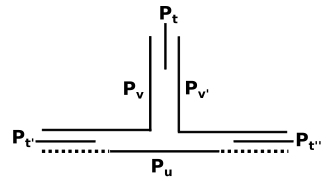
\includegraphics[width=5.5cm]{img/clawGrid} & &
    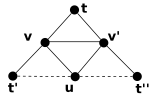
\includegraphics[width=3.5cm]{img/clawInduced.png}
    \\
    \footnotesize %\centering 
    (a)  \footnotesize Claw with paths. && \footnotesize (b) Subgraph induced by paths.\\
  \end{tabular}

 \caption{Reconstruction of the intersection model.}
 \label{fig:clawGrid}
\end{figure} 

 


% \begin{figure}[h]
%   \centering
%   \begin{tabular}{  c p{0.7cm} c}
%     %\centering
%     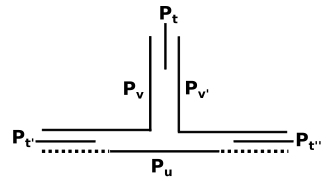
\includegraphics[width=5.5cm]{img/clawGrid} & &
%     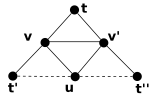
\includegraphics[width=3.5cm]{img/clawInduced.png}
%     \\
%     \footnotesize %\centering 
%     (a)  \footnotesize Clique-garra com caminhos adicionais. && \footnotesize (b) Subgrafo induzido pelos caminhos.\\
%   \end{tabular}

%  \caption{Reconstrução do modelo de intersecção.}
%  \label{fig:clawGrid}
% \end{figure} 

 



Note  que qualquer grafo toro-livre é $\{S_{3}, S_{3'}, S_{3''}\}$-livre, assim nosso resultado anterior implica no Lema 5 de~\cite{ries2009}.


\begin{figure}[h]
  \centering
  \begin{tabular}{  c p{0.7cm} c }
    \centering
    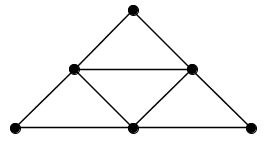
\includegraphics[width=4cm]{img/s3.png} & &
    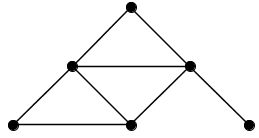
\includegraphics[width=4cm]{img/s3-1.png}
    \\
    \footnotesize \centering 
    (a)  \footnotesize Grafo $S_3$. &&  \footnotesize (b) Grafo $S_{3'}$. \\
    
    %---------------------
      \centering 
      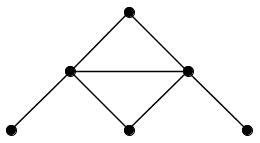
\includegraphics[width=4cm]{img/s3-2.png} & &
    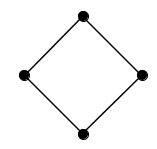
\includegraphics[width=3cm]{img/c4.png}
    \\
    \footnotesize \centering 
    (c)  \footnotesize Grafo $S_{3''}$. && \footnotesize (b) Grafo $C_{4}$.\\
  \end{tabular}

 \caption{Grafos do enunciado do  Teorema~\ref{lem:chordalDiamondFree}.}
 \label{fig:proibidos}
\end{figure} 



%--------------------------


O próximo teorema possui como consequência a identificação de algumas classes de grafos onde a existência de uma  representação $B_1$-EPG implica na existência de uma representação  $B_1$-EPG-Helly.


\begin{theorem} \label{lem:b1DiamondFree}
 Se $G$ é um grafo $B_1$-EPG e diamante-livre então $G$ é um grafo $B_1$-EPG-Helly.
 \end{theorem}

\begin{proof}
Se $G$ não é um grafo $B_1$-EPG-Helly, então em cada representação $B_1$-EPG de $G$, existe pelo menos uma clique que é representada como clique-garra e não como clique-aresta.  Considere qualquer representação $B_1$-EPG de $G$  e seja $K$ uma clique maximal que é representada como uma clique-garra. Assuma, sem perda de generalidade, que $K$ está sobre uma garra da grade com base $[x_0, x_2]\times\{y_0\}$ e centro $C = (x_1, y_0)$. Denote por  $\mathcal{P}_K$ o conjunto de caminhos correspondendo aos vértices de $K$. 
 Pelo Lema~\ref{lem:b1epgDiamondFree},  %(see~\cite{ries2009})
%no path $P_w$ for $w\notin K$ covers 
o segmento da grade $[x_0, x_2]\times\{y_0\}$ é coberto somente por vértices de $K$. % because $G$ is $C_4$-livre
 Para todo  ${\displaystyle \lrcorner}$-caminho %$P_v \in \mathcal{P}_K$ 
 (resp. ${\displaystyle \llcorner}$-caminho 
% $P_{v'} \in \mathcal{P}_K$
 ) pertencente a  $\mathcal{P}_K$, fazemos o seguinte: se %$P_v$ (resp. $P_{v'}$)
 o caminho não intersecta qualquer caminho $P_t \notin\mathcal{P}_K$ sobre a coluna $x_1$, então deletamos seu segmento vertical e adicionamos na grade o segmento $[x_1, x_2]\times\{y_0\}$ (resp. $[x_0, x_1]\times\{y_0\}$). Se depois dessa transformação não existir mais nenhum ${\displaystyle \lrcorner}$-caminhos (resp. ${\displaystyle \llcorner}$-caminhos) em $\mathcal{P}_K$, então terminamos, uma vez que temos obtido uma clique-aresta. Agora, podemos assumir que todo  ${\displaystyle \lrcorner}$-caminho   e todo ${\displaystyle \llcorner}$-caminho em $ \mathcal{P}_K$ intersecta algum caminho $P_t \notin \mathcal{P}_K$   sobre a coluna $x_1$ (note que podemos assumir que é o mesmo caminho $P_t$ para todos os vértices). Uma vez que $K$ é clique-garra, existe um caminho $P_u \in \mathcal{P}_K$ cobrindo a base da garra. Assim, $G[v, v', u, t]$ induz um diamante, uma contradição.
\end{proof}  

Um \textit{conjunto independente} de vértices é um conjunto de vértices não dois a dois adjacentes.
Um grafo $G$ é dito ser \textit{Bipartido} se seu conjunto de vértices pode ser particionado em dois conjuntos independentes distintos.
 Existem grafos Bipartidos que não são grafos $B_1$-EPG, por exemplo o grafo $K_{2,5}$ e $K_{3,3}$ (veja explicação em~\cite{cohen2014}). Claramente, uma vez que grafos Bipartidos são triângulo-livre, qualquer representação $B_1$-EPG de um grafo Bipartite é também uma representação $B_1$-EPG-Helly.
 Um resultado similar (mas um pouco mais fraco) é obtido como corolário do teorema anterior.


\begin{corollary}
Se $G$ é um grafo Bipartido $B_1$-EPG então $G$ é um grafo $B_1$-EPG-Helly.
\end{corollary}

\begin{proof}
Os grafos Bipartidos são diamante-livre, assim pelo Teorema~\ref{lem:b1DiamondFree} esses grafos são grafos $B_1$-EPG-Helly.
\end{proof}

Um \textit{grafo Bloco } ou \textit{grafo Árvore Clique} é um tipo de grafo em que toda componente biconexa (bloco) é uma clique.

\begin{corollary}\label{lem:cdf}
 Grafos Bloco são $B_1$-EPG-Helly.
\end{corollary}

\begin{proof}
Grafos Bloco são conhecidos por corresponderem exatamente à classe de grafos Cordal diamante-livre, assim pelo Teorema 19 de \cite{ries2009}, todos grafos Bloco são grafos  $B_1$-EPG. Segue do Teorema~\ref{lem:b1DiamondFree} que todos grafos Bloco estão na classe de grafos $B_1$-EPG-Helly. 
\end{proof} 

Um \textit{grafo Cactus} (algumas vezes chamado também de Árvore Cactus) é um grafo conexo em que quaisquer dois ciclos possuem no máximo um vértice em comum. Equivalentemente, ele é um grafo conexo em que toda aresta pertence a no máximo um ciclo, ou (para um cactus não trivial) em que cada bloco (subgrafo maximal sem vértice de corte) é uma aresta ou um ciclo. A família de grafos em que cada componente é um Cactus é fechada sob operações menores de grafos. Essa família de grafos pode ser caracterizada por um único subgrafo proibido menor, o grafo diamante.
 
\begin{corollary}
Grafos Cactus são  $B_1$-EPG-Helly.
\end{corollary}
\begin{proof}
Em~\cite{cela2019monotonic} foi provado que todo grafo Cactus graph é um grafo  $B_1$-EPG monotônico 
(existe uma representação $B_1$-EPG onde todos os caminhos são ascendentes em linhas e colunas). 
Assim, grafos Cactus são grafos $B_1$-EPG. 

Uma vez que Cactus são diamante-livre, pelo Teorema~\ref{lem:b1DiamondFree}, a prova segue verdadeira.
\end{proof}

Dado um grafo $G$, seu \textit{grafo Linha} $L(G)$ é um grafo tal que cada vértice de $L(G)$ representa uma aresta de  $G$ e dois  vértices de $L(G)$ são adjacentes se e somente se suas arestas correspondentes compartilham um vértice comum (i.e. elas ``são incidentes'' em um mesmo vértice) em $G$.  
Um grafo $G$ é um \textit{grafo Linha de um grafo Bipartido} (ou simplesmente \textit{Linha de Bipartido}) se e somente se ele não contem  garra, nem ciclo ímpar, e nem diamante como subgrafo induzido, \cite{harary1974line}.



\begin{corollary}\label{coro:lineOfBipartido}
 Grafos Linha de Bipartido são $B_1$-EPG-Helly. 
\end{corollary}

\begin{proof}
Grafos Linha de Bipartido foram provados ser $B_1$-EPG in~\cite{golumbic2018edge}. Uma vez que eles são diamante-livre, a prova segue diretamente pelo Teorema~\ref{lem:b1DiamondFree}.
\end{proof}

O diagrama da Figura~\ref{fig:diagram}
ilustra o relacionamento de continência entre as classes de grafos estudadas até agora neste trabalho.  
Listamos na Figura~\ref{fig:exemplosDiagram} exemplos de grafos em cada região numerada do diagrama. Os números de cada item abaixo correspondem às respectivas regiões com mesmo número do diagrama ilustrado na Figura~\ref{fig:diagram}.

%This numbers correspond with the respective number item and in some cases we make a brief explanation.

 \begin{figure}[htb]	
 \center%6.3
 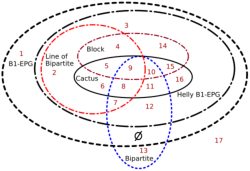
\includegraphics[width=8cm]{./img/diagram.pdf}
 \caption{Diagrama de algumas classes de grafos.}
\label{fig:diagram}
\end{figure}  
 

\begin{enumerate}[label=(\arabic*)]
    \item Grafos $B_1$-EPG  - $B_1$-EPG-Helly, ilustrado na Figura~\ref{fig:exemplosDiagram}(a), grafo $E_1$;%1
    
    \item Grafos Linha de Bipartido  - Cactus - Bloco - Bipartido, ilustrado na Figura~\ref{fig:exemplosDiagram}(b), grafo $E_2$;%2
    \item Grafos $B_1$-EPG-Helly - Linha de Bipartido - Bloco - Cactus - Bipartido, ilustrado na Figura~\ref{fig:exemplosDiagram}(c), grafo $E_3$;%3
    \item Grafos Bloco $\cap$ Linha de Bipartido - Cactus - Bipartido, ilustrado na Figura~\ref{fig:exemplosDiagram}(d), grafo $E_4$;%4
    \item Grafos Bloco $\cap$ Linha de Bipartido $\cap$  Cactus - Bipartido, ilustrado na Figura~\ref{fig:exemplosDiagram}(e), grafo $E_5$;%5
    \item Grafos Cactus $\cap$ Linha de Bipartido - Bloco - Bipartido. Essa intersecção é vazia. Seja $G$ um grafo que é um Cactus e Linha de Bipartido então $G$ é $\{$garra, ciclo ímpar, diamante$\}$-livre. Mas $G$ não é um grafo Bipartido, então $G$ possui um ciclo ímpar, o que é um absurdo considerando a hipótese de que $G$ é Linha de Bipartido; %Dessa forma $G$ possui no mínimo um triângulo ou ciclo ímpar  $C_n, n\geq 4$, e $G$ também é um grafo conexo. Mas dado um ciclo $C_n, n\geq 4$, ao adicionar um terceiro vértice adjacente a qualquer vértice desse ciclo então isso induz uma garra, 
    %absurd with the hypothesis of $G$ is Linha de Bipartido;%6
    \item Grafos Bipartido $\cap$ Linha de Bipartido  - Cactus - grafos Bloco, ilustrado na Figura~\ref{fig:exemplosDiagram}(f), grafo $E_7$;%7
    \item Grafos Bipartido $\cap$ Linha de Bipartido $\cap$  Cactus - grafos Bloco, ilustrado na Figura~\ref{fig:exemplosDiagram}(g), grafo $E_8$;%8
    \item Grafos Bipartido $\cap$ Linha de Bipartido $\cap$  Cactus $\cap$ grafos Bloco, ilustrado na Figura~\ref{fig:exemplosDiagram}(h), grafo $E_9$;%9
  \item Grafos Bipartido $\cap$  Cactus $\cap$ Bloco - Grafos Linha de Bipartido, ilustrado na Figura~\ref{fig:exemplosDiagram}(i), grafo $E_{10}$;%10
    \item Grafos Bipartido  $\cap$  Cactus - Bloco -  Grafos Linha de Bipartido, ilustrado na Figura~\ref{fig:exemplosDiagram}(j), grafo $E_{11}$;%11
     \item Grafos Bipartido $\cap$ $B_1$-EPG-Helly - Cactus - Bloco -  Grafos Linha de Bipartido, ilustrado na Figura~\ref{fig:exemplosDiagram}(k), grafo $E_{12}$;%12
      \item Grafos Bipartido - $B_1$-EPG, ilustrado na Figura~\ref{fig:exemplosDiagram}(l), grafo $E_{13}$;%13
      \item Grafos Bloco - Bipartido - Linha de Bipartido  - Cactus, ilustrado na Figura~\ref{fig:exemplosDiagram}(m), grafo $E_{14}$;%14
 
      \item Grafos Bloco $\cap$  Cactus -  Linha de Bipartido - Bipartido, ilustrado na Figura~\ref{fig:exemplosDiagram}(n), grafo $E_{15}$;%15
      \item Grafos Cactus - Bloco -  Linha de Bipartido - Bipartido, ilustrado na Figura~\ref{fig:exemplosDiagram}(o), grafo $E_{16}$, os ciclos ímpares $C_{2n+1},n\geq 2$;%16
      \item Grafos Helly EPG - $B_1$-EPG  - Bipartido, ilustrado na Figura~\ref{fig:exemplosDiagram}(p), grafo  $E_{17}$;%17
\end{enumerate}

 \begin{figure}[htb]	
 
   \centering
  \begin{tabular}{  c c c c  c}
    %\centering
    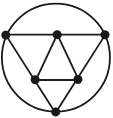
\includegraphics[width=2cm]{img/octaedroNoLabel.png} 
    & 
    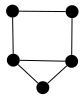
\includegraphics[width=1.5cm]{img/ex3.png} 
    & 
    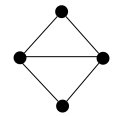
\includegraphics[width=2cm]{img/diamondNoLabel.png} 
    & 
    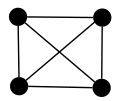
\includegraphics[width=1.5cm]{img/k4.png} 
    & 
    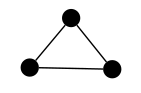
\includegraphics[width=2cm]{img/k3.png} 
    \\
    \footnotesize 
    (a)  \footnotesize Graph $E_1$. 
    & 
    \footnotesize (b) Graph $E_2$.
    & 
    \footnotesize (c) Graph $E_3$.
    & 
    \footnotesize (d) Graph $E_4$.
    & 
    \footnotesize (e) Graph $E_5$.
    \\%%Segunda linha
        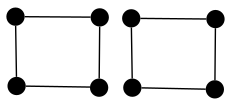
\includegraphics[width=2.5cm]{img/2c4.png} 
    & 
    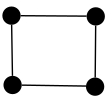
\includegraphics[width=1.5cm]{img/c4e.png} 
    & 
    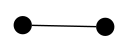
\includegraphics[width=1.8cm]{img/k2.png} 
    & 
    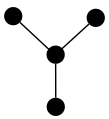
\includegraphics[width=1cm]{img/e10.png} 
    & 
    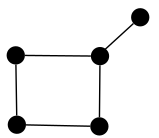
\includegraphics[width=1.8cm]{img/e11.png} 
    \\ %%Segundo Bloco legendas
    \footnotesize 
    (f)  \footnotesize Graph $E_7$. 
    & 
    \footnotesize (g) Graph $E_8$.
    & 
    \footnotesize (h) Graph $E_9$.
    & 
    \footnotesize (i) Graph $E_{10}$.
    & 
    \footnotesize (j) Graph $E_{11}$.
    %%Terceira linha de imagens
    \\%%Terceira linha
        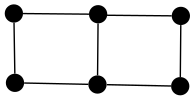
\includegraphics[width=2.5cm]{img/e12.png} 
    & 
    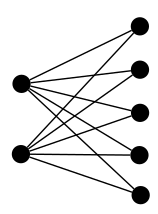
\includegraphics[width=2cm]{img/k25.png} 
    & 
    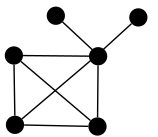
\includegraphics[width=2cm]{img/e14.png} 
    & 
    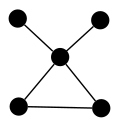
\includegraphics[width=1.8cm]{img/e15.png} 
    & 
    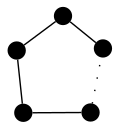
\includegraphics[width=1.8cm]{img/c2n+1.png} 
    \\ %%Terceiro Bloco legendas
    \footnotesize 
    (k)  \footnotesize Graph $E_{12}$. 
    & 
    \footnotesize (l) Graph $E_{13}$.
    & 
    \footnotesize (m) Graph  $E_{14}$.
    & 
    \footnotesize (n) Graph $E_{15}$.
    & 
    \footnotesize (o)  Graph $E_{16}$,  $C_{2n+1},n\geq2$.
    \\
    &&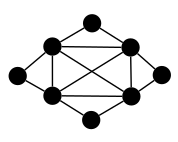
\includegraphics[width=2.5cm]{img/4sunNoLabel.png}&&
    \\
    &&\footnotesize (p)  Graph $E_{17}$.&&
    
    %\multicolumn{3}{c}{ \footnotesize (c) Another partial single bend representation of $H$ } \\
  \end{tabular}
 \caption{The set of instances for Venn Diagram of the graph classes of this paper.}
 %, see  more in~\cite{leveque2009characterizing,tondato2009grafos}
 \label{fig:exemplosDiagram}
\end{figure}  
 



















%  \begin{figure}[htb]	
 
%   \centering
%   \begin{tabular}{  c c c c  c}
%     %\centering
%     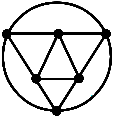
\includegraphics[width=1.7cm]{img/octaedro2.png} 
%     & 
%     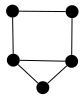
\includegraphics[width=1.5cm]{img/ex3.png} 
%     & 
%     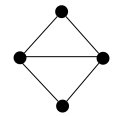
\includegraphics[width=2cm]{img/diamondNoLabel.png} 
%     & 
%     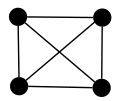
\includegraphics[width=1.5cm]{img/k4.png} 
%     & 
%     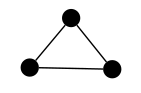
\includegraphics[width=2cm]{img/k3.png} 
%     \\
%     \footnotesize 
%     (a)  \footnotesize Grafo $E_1$. 
%     & 
%     \footnotesize (b) Grafo $E_2$.
%     & 
%     \footnotesize (c) Grafo $E_3$.
%     & 
%     \footnotesize (d) Grafo $E_4$.
%     & 
%     \footnotesize (e) Grafo $E_5$.
%     \\%%Segunda linha
%         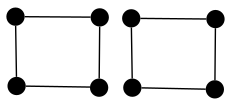
\includegraphics[width=2.5cm]{img/2c4.png} 
%     & 
%     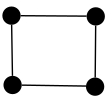
\includegraphics[width=1.5cm]{img/c4e.png} 
%     & 
%     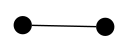
\includegraphics[width=1.8cm]{img/k2.png} 
%     & 
%     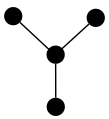
\includegraphics[width=1cm]{img/e10.png} 
%     & 
%     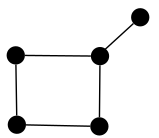
\includegraphics[width=1.8cm]{img/e11.png} 
%     \\ %%Segundo Bloco legendas
%     \footnotesize 
%     (f)  \footnotesize Grafo $E_7$. 
%     & 
%     \footnotesize (g) Grafo $E_8$.
%     & 
%     \footnotesize (h) Grafo $E_9$.
%     & 
%     \footnotesize (i) Grafo $E_{10}$.
%     & 
%     \footnotesize (j) Grafo $E_{11}$.
%     %%Terceira linha de imagens
%     \\%%Terceira linha
%         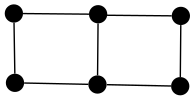
\includegraphics[width=2.5cm]{img/e12.png} 
%     & 
%     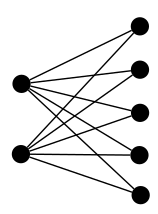
\includegraphics[width=2cm]{img/k25.png} 
%     & 
%     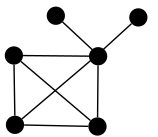
\includegraphics[width=2cm]{img/e14.png} 
%     & 
%     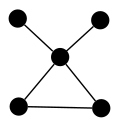
\includegraphics[width=1.8cm]{img/e15.png} 
%     & 
%     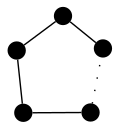
\includegraphics[width=1.8cm]{img/c2n+1.png} 
%     \\ %%Terceiro Bloco legendas
%     \footnotesize 
%     (k)  \footnotesize Grafo $E_{12}$. 
%     & 
%     \footnotesize (l) Grafo $E_{13}$.
%     & 
%     \footnotesize (m) Grafo  $E_{14}$.
%     & 
%     \footnotesize (n) Grafo $E_{15}$.
%     & 
%     \footnotesize (o)  Grafo $E_{16}$,  $C_{2n+1},n\geq2$.
%     \\
%     &&\includegraphics[width=2.5cm]{img/4sunNoLabel.png}&&
%     \\
%     &&\footnotesize (p)  Grafo $E_{17}$.&&
    
%     %\multicolumn{3}{c}{ \footnotesize (c) Another partial single bend representation of $H$ } \\
%   \end{tabular}
%  \caption{O conjunto de instâncias para o diagrama de Venn das classes de grafos estudadas até aqui.}
%  %, see  more in~\cite{leveque2009characterizing,tondato2009grafos}
%  \label{fig:exemplosDiagram}
% \end{figure}  
 

\section{Relacionamento de Contenção entre Grafos Cordal $B_1$-EPG, VPT e EPT}


 Qualquer grafo que admite uma representação $B_1$-EPG  cujos caminhos não cobrem todas as arestas de um polígono da grade  (i.e. o grafo subjacente da grade é uma árvore) é também um grafo EPT: a mesma representação é ao mesmo tempo uma representação $B_1$-EPG e $EPT$.
Todavia, é fácil verificar que o grafo subjacente da grade de qualquer representação $B_1$-EPG de um ciclo $C_n$ com  $n\geq 5$ não é uma árvore,
%has a non Cordal subjacent grade subgraph 
apesar de $C_n$ ser um grafo  EPT. Nosso objetivo de médio prazo é compreender os grafos $B_1$-EPG que são também grafos  EPT. Quando uma representação $B_1$-EPG pode ser reorganizada de forma a se tornar uma representação EPT? Nessa seção, responderemos essa questão para os grafos   Cordal $B_1$-EPG e de fato provamos que todo grafo Cordal $B_1$-EPG é EPT. Antes de conseguir esse resultado tivemos algumas tentativas sem sucesso para demonstrar que para um dado grafo $G$ com uma representação $B_1$-EPG cujos caminhos cobrissem todas arestas de algum polígono da  grade, e tentando mostrar que se nenhum dos caminhos pudesse ser modificado de forma a evitar uma aresta do polígono, então   $G$ teria algum ciclo sem corda (i.e. $G$ não seria Cordal).  Nossa surpresa foi que a única forma que encontramos de demonstrar o principal Teorema~\ref{teo:b1epgept} foi através dos grafos $VPT$.

 A partir de agora, provaremos o seguinte teorema.

\begin{theorem}\label{teo:CordalB1inVPT}
Cordal $B_1$-EPG $\subsetneq$ VPT. 
\end{theorem}

Em~L{\'e}v{\^e}que et al. \cite{leveque2009characterizing} apud \cite{alcon2015characterizing} os grafos VPT foram caracterizados por uma família minimal de subgrafos induzidos proibidos,
os quais estão representados na
Figura~\ref{fig:16proibidos} mais o ciclo induzido  $C_n$ para $n\geq 4$. Portanto, de forma a provar que os grafos Cordal $B_1$-EPG estão em VPT é suficiente mostrar que nenhum dos grafos na Figura~\ref{fig:16proibidos} 
é $B_1$-EPG. Utilizaremos esta abordagem. %The following lemmas are developed with that objective.   

Primeiro, note que em cada um dos grafos $F_{1}, F_{2}, F_{3}, F_{4}$ e $F_{5}$ ( Figuras~\ref{fig:16proibidos}(a), (b), (c), (d), (e), respectivamente), a vizinhança do  vértice universal (o vértice que está destacado e maior que os outros, nas respectivas Figuras) contem uma  tripla asteroidal. Portanto, pelo Lema~\ref{l:AT-livre}, esses grafos não estão em  $B_1$-EPG.

Agora, em cada um dos grafos $F_{11}, F_{12}, F_{13}, F_{14}$, $F_{15}$ e $F_{16}$  (Figuras~\ref{fig:16proibidos}(k), (l), (m), (n), (o), (p), respectivamente), seja $C$ a clique maximal em destaque negrito. É fácil checar que, em todos os casos, o grafo branch $B(G|C)$ contem um ciclo induzido $C_n$, para algum  $n\geq 4$, ou um caminho induzido $P_6$; assim, pelo  Lema~\ref{l:branch}, os grafos $F_{11}, F_{12}, F_{13}, F_{14}$, $F_{15}$ e $F_{16}$ não estão em $B_1$-EPG.



Um \textit{satélite} de uma clique $K$ é um vértice $v$ tal que $B_v=N(v)\cap K$ é um
subconjunto próprio não vazio de  $K$. O conjunto $B_v$ é chamado de \textit{base} de $v$ e  ela é dito ser \textit{minimal} se nenhuma outra base de um satélite de $K$ está propriamente contida em $B_v$, ver~\cite{alcon2010necessary}.

 Seja $I=[q_1,q_2]$ o intervalo da grade definido pela intersecção $\displaystyle \cap_{v\in K}P_v$, onde $K$
é uma clique-aresta de um grafo $G$. Para qualquer $v\in K$, pela remoção do intervalo $(q_1,q_2)$, o caminho $P_v$
é dividido em duas \textit{partes disjuntas}: \textit{parte 1}  contendo  $q_1$, e  \textit{parte 2}  contendo $q_2$.
Se $w$  é um satélite de $K$ adjacente a $v$, então $P_w\cap P_v$ está contido na parte 1 ou na parte 2 de $P_v$. Diremos que  $P_w$ intersecta $P_v$ no lado 1 ou no lado 2 se ele intersecta na parte 1 ou na parte 2, respectivamente.  Note  que se $w$  também é adjacente a outro vértice $v'$ de $K$, então  $P_w$ intersecta $P_v$ e $P_{v'}$ sobre o mesmo lado de $K$. Isso nos permite dividir os satélites de $K$ em dois \textit{grupos disjuntos}, os que estão do  \textit{lado 1} de $K$ e os que estão do \textit{lado 2}.

%%%%%%%%%%%%%%%%%%%%%%%%%%%
\begin{fac} \label{f:between}Sejam $e_1$, $e_2$ e $e_3$  três arestas distintas de um caminho com uma dobra $P$, e assuma que $e_2$ está entre  $e_1$ e $e_3$ sobre $P$. Se $P_1$ e $P_3$ são caminhos com uma dobra tal que: $P_1$ contem $e_1$, $P_3$ contem $e_3$, e  $P_1$ e $P_3$ intersectam-se em no mínimo uma aresta, então $P_1$ ou $P_3$ contem $e_2$.
\end{fac}
%%%%%%%%%%%%%%%%%%%%%%%%%%%%%%

\begin{lema}\label{coro:3Cliques1EdgeClique}
Seja $G$ um grafo cujo conjunto de vértice pode ser particionado em uma  clique $K$ e um conjunto independente $I=\{w_1,w_2,w_3\}$,  tal que cada vértice de $K$ é adjacente a cada vértice de $I$.  Seja $K_i$ cada clique maximal   $K_i = K \cup w_i$, com $1 \leq i \leq 3$.
Em qualquer representação $B_1$-EPG de $G$, uma dessas cliques, digamos $K_2$, é uma clique-aresta, e seus dois  satélites $w_1$ e $w_3$ estão em lados diferentes.
\end{lema}

\begin{proof}
%%%%%%%%%%%%%%%%%%%%%%%%%%%%%%%
Seja $v$ qualquer vértice de $K$. Para $i\in \{1,2,3\}$, seja $I_{v,i}$ o subcaminho de  $P_v$
definido para ser $P_v\cap P_{w_i}$ (relembrando que consideramos o caminho como um conjunto de arestas). Claramente, os três subcaminhos são mutuamente aresta-disjuntos. Assim, sem perda de generalidade, por simetria, podemos assumir que 
$I_{v,2}$ está entre $I_{v,1}$ e $I_{v,3}$. Afirmamos que a clique $K_2$ é uma clique-aresta.
De fato, se ela não o é, % then $P_4$ contains no edge of the subpath $I_{1,4}$. And,
pelo Lema~\ref{lem:3cliquesNotgarra}, podemos assumir, também sem perda de generalidade, que $K_1$ é uma clique-aresta, o que implica que existe uma aresta  de $I_{v,1}$ coberta por todos os vértices de $K_1$.  Seja $q$ o centro da garra correspondendo à clique $K_2$; claramente $q$ é um ponto de $I_{v,2 }$. Uma vez que todos os vértices de $K$ devem conter $q$, porém nem todos eles podem cobrir a mesma aresta de $I_{v,2}$, we have that $q$ must be the extreme of  $I_{v,2}$ closest to  $I_{v,1}$. Therefore, if we let $e_1$ and $e_2$ be the two edges of $P_v$ incident on $q$ ($e_2$ the one contained in $I_{v,2}$),
we have that  all the vértices of $K$
contain  $e_1$ and at least one vértice of $K$, say $w$,  does not contain $e_2$. Observe this contradicts Fact \ref{f:between} (let $P_1=P_w$, $P_3=P_{w_3}$ and $e_3$ any edge of $I_{v,3}$. We conclude that $K_2$ is an clique-aresta; since $w_1$ and $w_3$ are satélites of $K_2$ the proof is complete. 

%%%%%%%%%%%%%%%%%%%%%%%%%%%%%%%%%%%%%%%%%%%%%%%
% By Lema~\ref{lem:3cliquesNotgarra} the clique maximal s $K_1, K_2$ and $K_3$ can not be represented simultaneously as clique-garras, thus at least one is clique-aresta, we say $K_2$. Since $G$ is a Cordal graph, then when $K_1$ and $K_3$ are represented as clique-garras they have  distinct centers.
% Given $\mathcal{P}_K$ the set of paths corresponding to the vértices of $K$. 
% Each clique-garra $K_i$ has at least one path $P_k \in \mathcal{P}_K$ that bend in this clique-garra. If all paths $P_k \in \mathcal{P}_K$ bend in some clique-garra then these paths can not bend in other clique-garra, i.e. if all paths $P_k \in \mathcal{P}_K$ bend in some clique-garra others cliques will be clique-aresta and the lemma holds. So, consider $K_1$ and $K_3$ as clique-garras.
% In each clique-garra $K_1, K_3$, either all paths $P_k \in \mathcal{P}_K$ intersect in some segment between center of clique-garra and right or left part of base, or then there is only one point of intersection of all paths (center of this garra, obviously) and there is no a representação $B_1$-EPG to $G$. Consider the first situation,  w.l.g. we say that $K_1$ has horizontal base in interval $(q_1,q_2)$ and that all paths $P_k \in \mathcal{P}_K$ intersect  at right of $q_2$. Then, $K_3$ with base in interval $(q_1'',q_2'')$ has same condition but with intersection of all paths at left of $q_1''$. Now we have a problem, if clique-aresta $K_2$ is at left of the center of the $K_1$ then there is a path $P_k \in \mathcal{P}_K$ that bend in the center of $K_1$ such that this path is not in $K_2$, the same is true if $K_2$ is at right of $K_3$. 
% Therefore, in this construction $K_2$ must be between the center of $K_1$ and $K_3$. 

% Thus there is always an clique-aresta $K_i$ located between two satélites $w_i$. 
\end{proof}
